\documentclass[1-ambra-tesi.tex]{subfiles}
 
\begin{document}
\label{sub:chapter3}

\begin{chapabstract}
\small{\lipsum[1]}\\

\begin{center}
    \noindent\makebox[0.8\linewidth]{\rule{0.8\paperwidth}{0.4pt}}
\end{center}
\vspace{2cm}
\end{chapabstract}


% ================================= CAPYBARAS ============

\lipsum[2]

\section{Let's talk about capybaras}
\label{sec:capybaras}

% wrapfigure example
\begin{wrapfigure}{l}{0.5\textwidth}
\centering
\captionsetup{width=\linewidth}
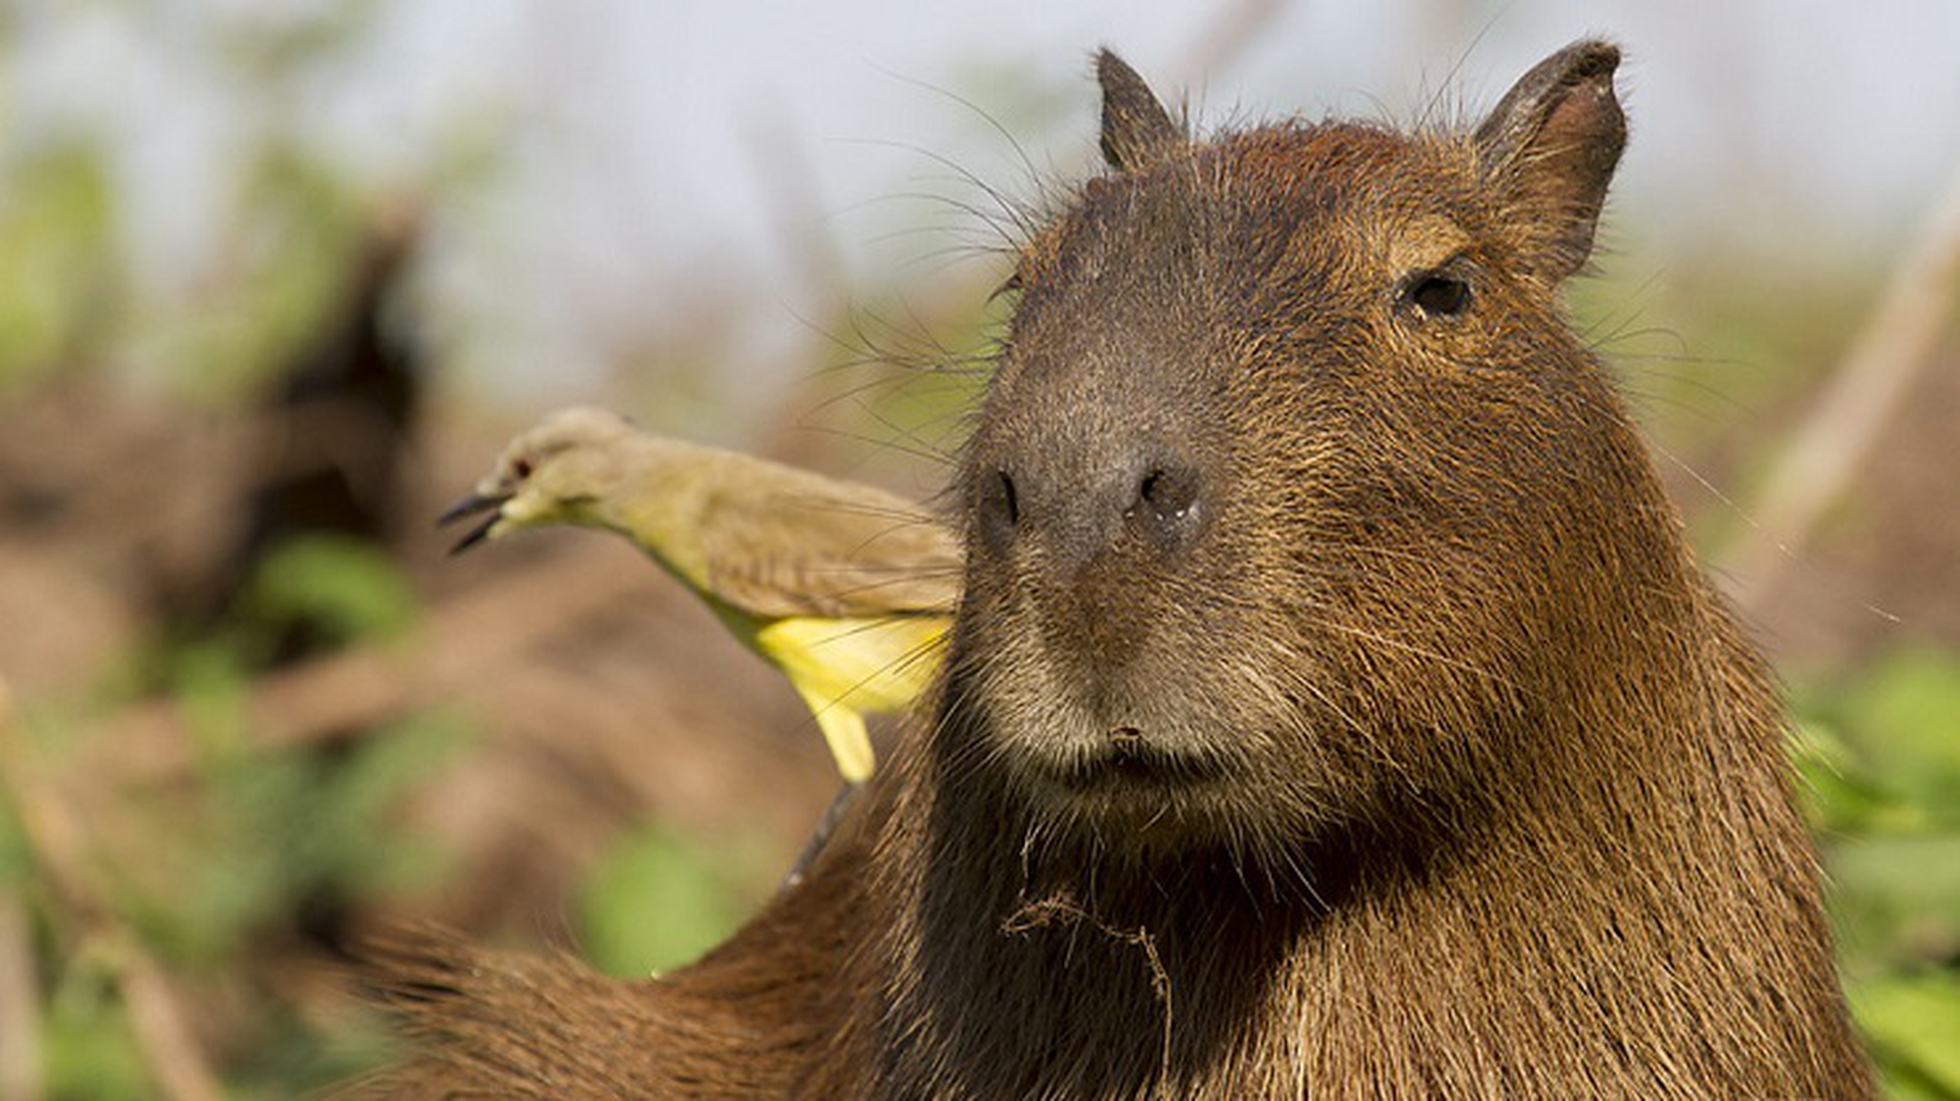
\includegraphics[width=\linewidth]{images/capybara.jpeg}
\caption{An hilarious capybara. \textbf{Credits:} the web.}
\label{fig:capybara}
\end{wrapfigure}

\lipsum[3]
\lipsum[4]\\

Refer to wrapfigure: \ref{fig:capybara}\\

\lipsum[5]

% fancy table
\begin{table}[ht]
    \centering
    \begin{tabular}{|c|c|c|c|c|}
    \multicolumn{5}{c}{\textbf{Fancy title here}}\\
    \hline
    \hline
    One                  & Two & Three & Four & Five \\
    \hline
    1                    & 2   & 3     & 4   & 5     \\
    1                    & 2   & 3     & 4   & 5     \\
    \hline
    \multirow{2}{*}{One} & 2   & 3     & 4   & 5     \\
                         & 2   & 3     & 4   & 5     \\
    \hline
    \end{tabular}
\caption{Fancy table.}
\label{tab:capybara}
\end{table}

\lipsum[6]\\

Refer to table: \ref{tab:capybara}.\\

\lipsum[7]

\end{document}

